\chapter{Data Structures}
\label{chp:datastrucutres}
A \textbf{data structure} is a data organization, management, and storage format that enables efficient access and modification of the collected data. The relationship among collected data, their properties, the operations that can be done on them, are all properties of the data structure \cite{wikidatastructure} (\href{https://en.wikipedia.org/wiki/Data_structure}{Data Structure, Wikipedia}). Data structure is the basis for an \textbf{abstract data type (ADT)}, a mathematical model for a \textbf{data type} \cite{wikidatatype} (\href{https://en.wikipedia.org/wiki/Data_type}{Data Type, Wikipedia}), which is defined by its behavior from the point of view of a user, its type of data, specifically in terms of possible values, by possible operations on these data, and by the behavior of these operations. This mathematical model contrasts with data structures, which are concrete representations of data, and are the point of view of an implementer, not of a user \cite{wikiabstractdatatype} (\href{https://en.wikipedia.org/wiki/Abstract_data_type}{Abstract Data Type, Wikipedia}).
\\
In this chapter the most important data structures like \textbf{collections}, \textbf{lists}, \textbf{arrays}, \textbf{linked lists}, \textbf{stacks}, and \textbf{queues} are introduced. For each data structure are shown all the most important properties, operations, and implementations.
\section{Collection}
A \textbf{collection} is an object that groups several different elements in only single unit. Collections are used to save, to find, to manipulate, and to communicate grouped data \cite{wikicollection} (\href{https://en.wikipedia.org/wiki/Collection_(abstract_data_type)}{Collection (abstract data type), Wikipedia}). Usually the elements belonging to a collection are of the same type, such as a poker hand (a collection of playing cards), a folder containing emails (a collection of emails), or a phone book (a map \textit{name} \(\rightarrow\) \textit{phone number}).
\section{List}
A \textbf{list} is a collection which represents a set of \textbf{ordered} elements, which can be also of different type. Same value elements can be repeated several times. Lists do not have a fixed size, and it is possible to add, to remove, and to modify all the elements in the list. The complexity of adding or removing an element is constant (\(O(1)\)).
\section{Array}
An \textbf{array} is a collection of elements of the same or also different type, in which each of them is identified with at least one \textbf{array index} or \textbf{key} \cite{wikiarray} (\href{https://en.wikipedia.org/wiki/Array_data_structure}{Array data structure, Wikipedia}). In some programming languages arrays have a fixed size, in others instead is fixed.
\begin{figure}[H]
	\begin{center}
		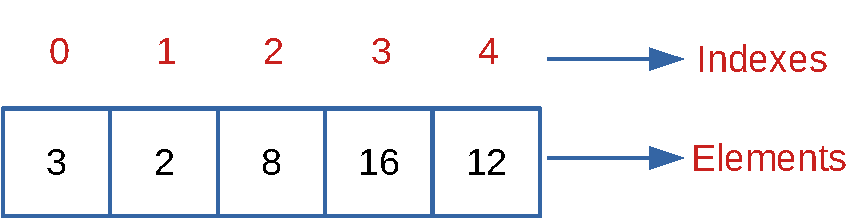
\includegraphics[scale=0.6]{chapters/datastructures/images/array_1.pdf}
		\caption[An example of an array with elements and indexes.]{An example of an array with elements and indexes.}
		\label{array_1}
	\end{center}
\end{figure}

\begin{figure}[H]
\centering
\tikzset{
mymat/.style={
  matrix of math nodes,
  text height=2.5ex,
  text depth=0.75ex,
  text width=3.25ex,
  align=center,
  column sep=-\pgflinewidth
  },
mymats/.style={
  mymat,
  nodes={draw,fill=#1}
  }  
}
\begin{tikzpicture}[node distance = 5mm and 0mm,
start chain = A going right,
box/.style = {rectangle, draw, inner sep=1mm, outer sep=0mm,
              minimum size=7mm,
                 on chain=A},
LA/.style = {-{Straight Barb[flex=0]},
               thick, shorten >=1mm, shorten <=1mm,
               looseness=1.6}, >=latex, nodes in empty cells, thick]

\matrix[mymat, anchor=east, row 2/.style={nodes=draw}]
at (0.5,0)
(mat1)
{
0 & 1 & 2 & 3 & 4 \\
8 & 2 & 4 & 1 & 7 \\
};

\draw (mat1-1-5.east)--++(0:3mm) node [right]{Indices};
\draw (mat1-2-5.east)--++(0:3mm) node [right]{Elements};

\end{tikzpicture}
\caption[An example of an array with elements and indexes.]{An example of an array with elements and indexes.}
\label{array_1}
\end{figure}

For doing any allowed operation to an element of an array it is enough to know its index. 

Adding or removing an element of an array could be a very expensive operation. This is because when a change take place to an element all the following indexes must be updated (Figure \ref{array_2}). The worst case complexity is \(O(n)\), where \(n\) is the size of the array.
\begin{figure}[H]
	\begin{center}
		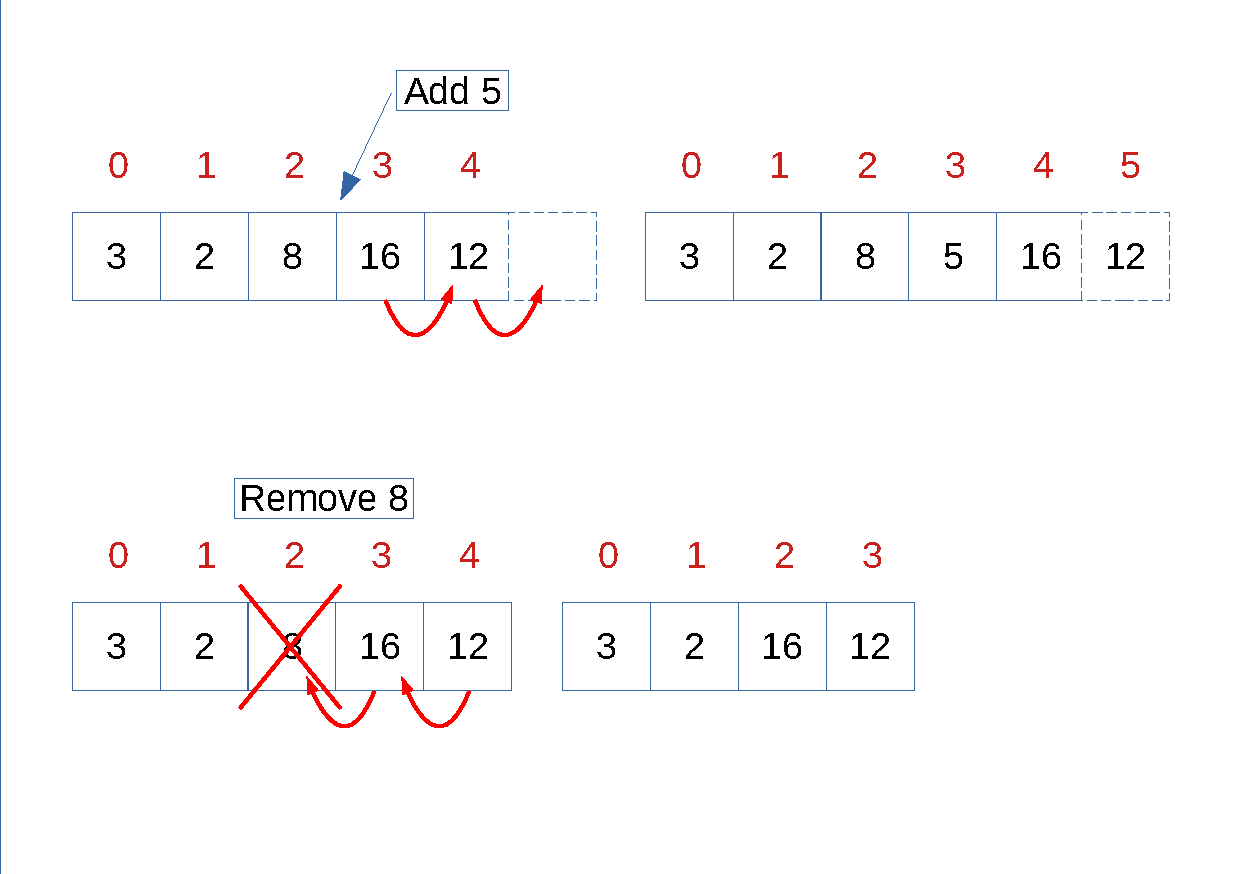
\includegraphics[scale=.6]{chapters/datastructures/images/array_2.pdf}
		\caption[Removing or adding an element from an array and the indexes update.]{Removing or adding an element from an array and the indexes update.}
		\label{array_2}
	\end{center}
\end{figure}

\begin{figure}[H]
\centering
\tikzset{
mymat/.style={
  matrix of math nodes,
  text height=2.5ex,
  text depth=0.75ex,
  text width=3.25ex,
  align=center,
  column sep=-\pgflinewidth
  },
mymats/.style={
  mymat,
  nodes={draw,fill=#1}
  }  
}
\begin{subfigure}[b]{\linewidth}
\centering
\begin{tikzpicture}[node distance = 5mm and 0mm,
start chain = A going right,
box/.style = {rectangle, draw, inner sep=1mm, outer sep=0mm,
              minimum size=7mm,
                 on chain=A},
LA/.style = {-{Straight Barb[flex=0]},
               thick, shorten >=1mm, shorten <=1mm,
               looseness=1.6}, >=latex, nodes in empty cells, thick]

\matrix[mymat, anchor=east, row 2/.style={nodes=draw}, 
        column 5/.style={nodes=densely dashed}]
at (0.5,0)
(mat1)
{
0 & 1 & 2 & 3 & \\
8 & 2 & 4 & 1 & \\
};
\matrix[mymat, anchor=west, row 2/.style={nodes=draw}, column 5/.style={nodes=densely dashed}] at (0.5,0)
(mat2)
{
0 & 1 & 2 & 3 & 4 \\
8 & 2 & 9 & 4 & 1 \\
};

\draw ($(mat1-2-3.north) + (-1mm, 10mm)$) node[draw=none, rectangle, align=left] (r1) {add 9};

\draw[->, >=stealth, BrickRed] (r1.south) -- (mat1-2-2.north east);

\path[->, >=stealth, BrickRed] (mat1-2-3.south) edge [bend right=60] node[draw=none] {} (mat1-2-4.south);
\path[->, >=stealth, BrickRed] (mat1-2-4.south) edge [bend right=60] node[draw=none] {} (mat1-2-5.south);

\end{tikzpicture}
\caption{Adding an element to an array.}
\label{adding_arr}
\end{subfigure}
%\hspace{1em}
\begin{subfigure}[b]{\linewidth}
\centering
\begin{tikzpicture}[node distance = 5mm and 0mm,
start chain = A going right,
box/.style = {rectangle, draw, inner sep=1mm, outer sep=0mm,
              minimum size=7mm,
                 on chain=A},
LA/.style = {-{Straight Barb[flex=0]},
               thick, shorten >=1mm, shorten <=1mm,
               looseness=1.6}, >=latex, nodes in empty cells, thick]

\matrix[mymat, anchor=east, row 2/.style={nodes=draw}] at (-1.4,0) (mat1)
{
0 & 1 & 2 & 3 \\
8 & 2 & 4 & 1 \\
};
\matrix[mymat, anchor=west, row 2/.style={nodes=draw}] at (-1.4,0)
(mat2)
{
0 & 1 & 2 \\
8 & 4 & 1 \\
};

\draw[BrickRed, style={-}] ($(mat1-2-2) + (-0.5,0.5)$) -- ($(mat1-2-2) + (0.5,-0.5)$);
\draw[BrickRed, style={-}] ($(mat1-2-2) + (0.5,0.5)$) -- ($(mat1-2-2) + (-0.5,-0.5)$);

\path[->, >=stealth, BrickRed] (mat1-2-4.south) edge [bend left=60] node[draw=none] {} (mat1-2-3.south);
\path[->, >=stealth, BrickRed] (mat1-2-3.south) edge [bend left=60] node[draw=none] {} (mat1-2-2.south);

\end{tikzpicture}
\caption{Removing an element to an array.}
\label{removing_arr}
\end{subfigure}
\caption[Adding \ref{adding_arr} or removing \ref{removing_arr} an element from an array and the indexes update.]{Adding \ref{adding_arr} or removing \ref{removing_arr} an element from an array and the indexes update.}
\label{array_2}
\end{figure}

\section{Linked List}
\label{linkedlist}
A \textbf{linked list} is a linear collection in which each element has the data and a reference to the next element (a link) \cite{wikilinkedlist} (\href{https://en.wikipedia.org/wiki/Linked_list}{Linked List, Wikipedia}). 
\begin{figure}[H]
	\begin{center}
		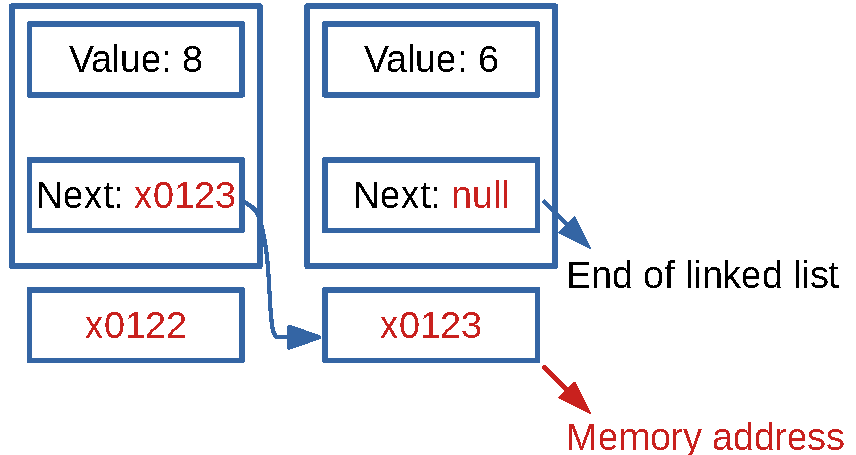
\includegraphics[scale=.6]{chapters/datastructures/images/linked_list_1.pdf}
		\caption[An example of a linked list with the data and the reference to the next element.]{An example of a linked list with the data and the reference to the next element.}
		\label{linked_list_1}
	\end{center}
\end{figure}

\begin{figure}[H]
\centering
\begin{tikzpicture}[double link/.style n args=2{on chain, rectangle split, rectangle split horizontal, rectangle split parts=2, draw, anchor=center, text height=1.5ex, node contents={#1\nodepart{two}#2},}, start chain=going right, >=stealth, thick, node distance=15mm]

\node[double link={$Head$}{\textcolor{BrickRed}{$0x00$}}, alias={h}];
\node[join={by ->}, double link={$7$}{\textcolor{BrickRed}{$0x01$}}, alias={a}];
\node[join={by ->}, double link={$1$}{\textcolor{BrickRed}{$0x02$}}, alias={b}];
\node[join={by ->}, double link={$13$}{\textcolor{BrickRed}{$null$}}, alias={c}];

\draw ($(a) + (0,-5mm)$) node[draw=none, rectangle, align=left] (r1) {\textcolor{BrickRed}{$0x00$}};
\draw ($(b) + (0,-5mm)$) node[draw=none, rectangle, align=left] (r2) {\textcolor{BrickRed}{$0x01$}};
\draw ($(c) + (0,-5mm)$) node[draw=none, rectangle, align=left] (r3) {\textcolor{BrickRed}{$0x02$}};

\draw ($(a) + (0,1)$) node[draw=none, rectangle, align=left] (r3) {Content};
\draw ($(a) + (4,1)$) node[draw=none, rectangle, align=left] (r4) {Address (pointer) of the next node};
\draw ($(c) + (2.4,0)$) node[draw=none, rectangle, align=left] (r5) {Last node \\ points to null};

\draw[->, >=stealth] (r3.south) -- (a.one north);
\draw[->, >=stealth] (r4.south) -- (a.two north);
\draw[->, >=stealth] (r5.west) -- (c.two east); 
\end{tikzpicture}

\caption[An example of a linked list with the data and the reference to the next element.]{An example of a linked list with the data and the reference to the next element.}
\label{linked_list_1}
\end{figure}

In a linked list the order of the elements is not assured. 

Operations like adding or removing an element in a linked list are very efficient, because it is enough to change the references of the elements involved in the operation. For example for adding a new element is enough to change the previous element reference to the just added element, and change the reference of the new element to the next element (Figure \ref{linked_list_2}). In case of removing an element it is enough to update the previous element's reference to the next element of the removed one (Figure \ref{linked_list_3}). 
\begin{figure}[H]
	\begin{center}
		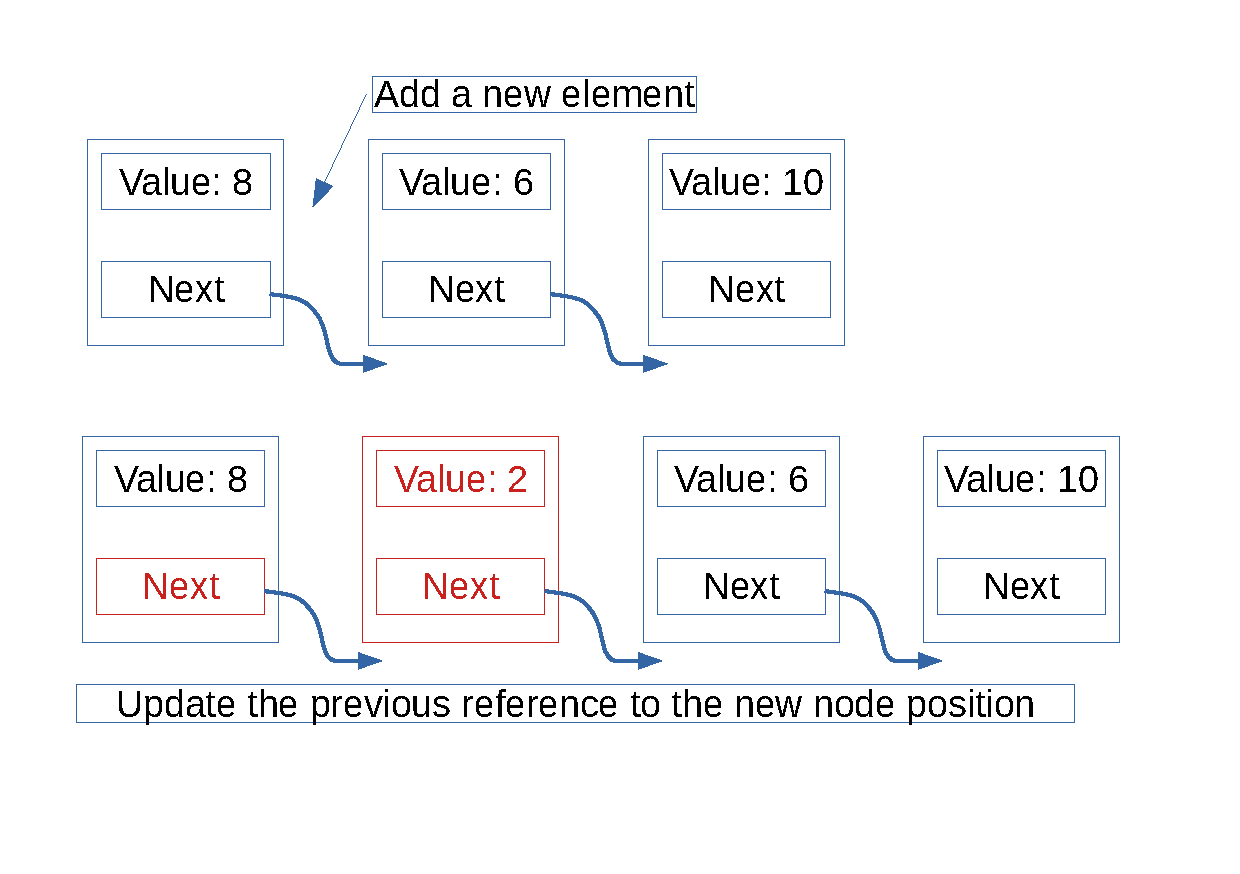
\includegraphics[scale=.6]{chapters/datastructures/images/linked_list_2.pdf}
		\caption[Adding a new element to a linked list.]{Adding a new element to the linked list. As explained before this operation is very efficient because it is enough to change the references of the new element and the previous element to the one just added.}
		\label{linked_list_2}
	\end{center}
\end{figure}

\begin{figure}[H]
\centering
\begin{tikzpicture}[double link/.style n args=2{on chain, rectangle split, rectangle split horizontal, rectangle split parts=2, draw, anchor=center, text height=1.5ex, node contents={#1\nodepart{two}#2},}, start chain=going right, >=stealth, thick, node distance=15mm]

\node[double link={$Head$}{\textcolor{BrickRed}{$0x00$}}, alias={h}];
\node[join={by ->}, double link={$7$}{\textcolor{BrickRed}{$0x01$}}, alias={a}];
\node[join={by ->}, double link={$1$}{\textcolor{BrickRed}{$0x02$}}, alias={b}];
\node[join={by ->}, double link={$13$}{\textcolor{BrickRed}{$null$}}, alias={c}];

\draw ($(a) + (0,-5mm)$) node[draw=none, rectangle, align=left] (r1) {\textcolor{BrickRed}{$0x00$}};
\draw ($(b) + (0,-5mm)$) node[draw=none, rectangle, align=left] (r2) {\textcolor{BrickRed}{$0x01$}};
\draw ($(c) + (0,-5mm)$) node[draw=none, rectangle, align=left] (r3) {\textcolor{BrickRed}{$0x02$}};
\draw ($(a) + (-5mm,10mm)$) node[draw=none, rectangle, align=left] (r4) {Add a new element};
\draw[->, >=stealth] (r4.south) -- (1.5,0);
\end{tikzpicture}

\begin{tikzpicture}[double link/.style n args=2{on chain, rectangle split, rectangle split horizontal, rectangle split parts=2, draw, anchor=center, text height=1.5ex, node contents={#1\nodepart{two}#2},}, start chain=going right, >=stealth, thick, node distance=15mm]

\node[double link={$Head$}{\textcolor{BrickRed}{$0x04$}}, alias={h}];
\node[join={by ->}, double link={$3$}{\textcolor{BrickRed}{$0x00$}}, alias={aa}, BrickRed];
\node[join={by ->}, double link={$7$}{\textcolor{BrickRed}{$0x01$}}, alias={a}];
\node[join={by ->}, double link={$1$}{\textcolor{BrickRed}{$0x02$}}, alias={b}];
\node[join={by ->}, double link={$13$}{\textcolor{BrickRed}{$null$}}, alias={c}];

\draw ($(aa) + (0,-5mm)$) node[draw=none, rectangle, align=left] (r11) {\textcolor{BrickRed}{$0x04$}};
\draw ($(a) + (0,-5mm)$) node[draw=none, rectangle, align=left] (r1) {\textcolor{BrickRed}{$0x00$}};
\draw ($(b) + (0,-5mm)$) node[draw=none, rectangle, align=left] (r2) {\textcolor{BrickRed}{$0x01$}};
\draw ($(c) + (0,-5mm)$) node[draw=none, rectangle, align=left] (r3) {\textcolor{BrickRed}{$0x02$}};
\end{tikzpicture}

\caption[Adding a new element to a linked list.]{Adding a new element to the linked list. As explained before this operation is very efficient because it is enough to change the references of the new element and the previous element to the one just added.}
\label{linked_list_2}
\end{figure}

\begin{figure}[H]
	\begin{center}
		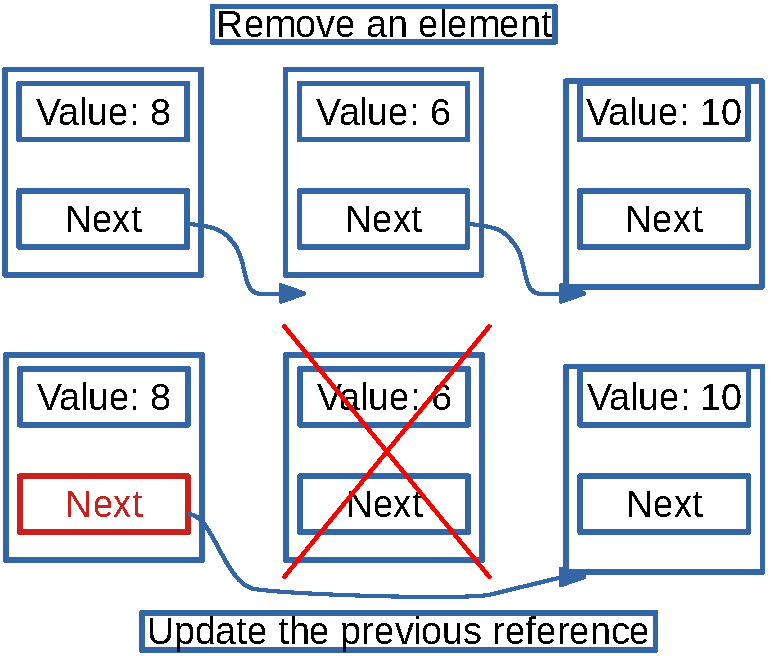
\includegraphics[scale=.6]{chapters/datastructures/images/linked_list_3.pdf}
		\caption[Removing an element to a linked list.]{Removing an element to a linked list.}
		\label{linked_list_3}
	\end{center}
\end{figure}

\begin{figure}[H]
\centering
\begin{tikzpicture}[double link/.style n args=2{on chain, rectangle split, rectangle split horizontal, rectangle split parts=2, draw, anchor=center, text height=1.5ex, node contents={#1\nodepart{two}#2},}, start chain=going right, >=stealth, thick, node distance=15mm]

\node[double link={$Head$}{\textcolor{BrickRed}{$0x00$}}, alias={h}];
\node[join={by ->}, double link={$7$}{\textcolor{BrickRed}{$0x01$}}, alias={a}];
\node[join={by ->}, double link={$1$}{\textcolor{BrickRed}{$0x02$}}, alias={b}];
\node[join={by ->}, double link={$13$}{\textcolor{BrickRed}{$null$}}, alias={c}];

\draw ($(a) + (0,-5mm)$) node[draw=none, rectangle, align=left] (r1) {\textcolor{BrickRed}{$0x00$}};
\draw ($(b) + (0,-5mm)$) node[draw=none, rectangle, align=left] (r2) {\textcolor{BrickRed}{$0x01$}};
\draw ($(c) + (0,-5mm)$) node[draw=none, rectangle, align=left] (r3) {\textcolor{BrickRed}{$0x02$}};

\draw[BrickRed, style={-}] ($(a) + (-0.5,0.5)$) -- ($(a) + (0.5,-0.5)$);
\draw[BrickRed, style={-}] ($(a) + (0.5,0.5)$) -- ($(a) + (-0.5,-0.5)$);
\end{tikzpicture}

\begin{tikzpicture}[double link/.style n args=2{on chain, rectangle split, rectangle split horizontal, rectangle split parts=2, draw, anchor=center, text height=1.5ex, node contents={#1\nodepart{two}#2},}, start chain=going right, >=stealth, thick, node distance=15mm]

\node[double link={$Head$}{\textcolor{BrickRed}{$0x01$}}, alias={h}];
\node[join={by ->}, double link={$1$}{\textcolor{BrickRed}{$0x02$}}, alias={b}];
\node[join={by ->}, double link={$13$}{\textcolor{BrickRed}{$null$}}, alias={c}];

\draw ($(b) + (0,-5mm)$) node[draw=none, rectangle, align=left] (r2) {\textcolor{BrickRed}{$0x01$}};
\draw ($(c) + (0,-5mm)$) node[draw=none, rectangle, align=left] (r3) {\textcolor{BrickRed}{$0x02$}};
\end{tikzpicture}

\caption[Removing an element to a linked list.]{Removing an element to a linked list.}
\label{linked_list_3}
\end{figure}

The complexity for adding or removing an element is constant \(O(1)\).
Linked lists can be also \textbf{doubly linked list} (Figure \ref{linked_list_4}), which evry element has the reference to the previous and next element of the collection \cite{wikidoublylinkedlist} (\href{https://en.wikipedia.org/wiki/Doubly_linked_list}{Doubly linked list, Wikipedia}).
\begin{figure}[H]
	\begin{center}
		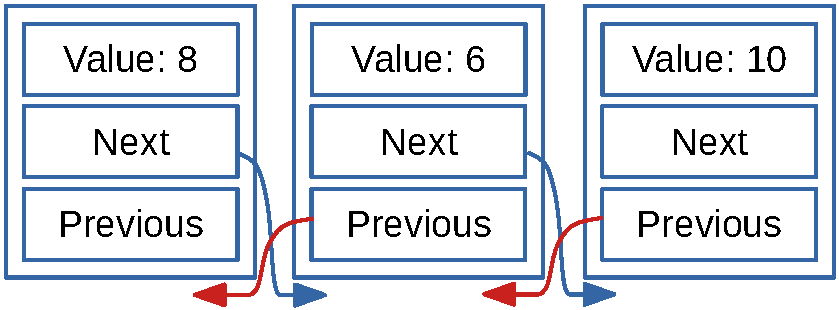
\includegraphics[scale=.6]{chapters/datastructures/images/linked_list_4.pdf}
		\caption[Doubly linked list.]{Doubly linked list.}
		\label{linked_list_4}
	\end{center}
\end{figure}

\begin{figure}[H]
\centering
\begin{tikzpicture}[list/.style={thick, rectangle split, rectangle split parts=3, draw, rectangle split horizontal, minimum size=18pt, inner sep=5pt, text=black}, ->, start chain, thick]

  \node[list, on chain] (a) {\nodepart{second} $7$};
  \node[list, on chain] (b) {\nodepart{second} $1$};
  \node[list, on chain] (c) {\nodepart{second} $13$};

  \node[draw, rectangle, minimum size=18pt] (d) [right=of c] {\textcolor{BrickRed}{$null$}};
  \node[draw, rectangle, minimum size=18pt] (e) [left= of a] {\textcolor{BrickRed}{$null$}};
  
  \draw[*->, >=stealth] ($(a.one) + (0.2, 0.1)$) -- (e.east);
   
  \path[*->] let \p1 = (a.three), \p2 = (a.center) in (\x1,\y2) edge [bend left] ($(b.one)+(0,0.2)$);
  \path[*->] ($(b.one)+(0.1,0.1)$) edge [bend left] ($(a.three)+(0,-0.05)$);
  \path[*->] let \p1 = (b.three), \p2 = (b.center) in (\x1,\y2) edge [bend left] ($(c.one)+(0,0.2)$);
  
  \draw[*->] let \p1 = (c.three), \p2 = (c.center) in (\x1,\y2) -- (d);
  \path[*->] ($(c.one)+(0.1,0.1)$) edge [bend left] ($(b.three)+(0,-0.05)$);
\end{tikzpicture}
\caption[Doubly linked list.]{Doubly linked list.}
\label{linked_list_4}
\end{figure}

Linked list are used for implementing other data structures such as lists, stacks, queues, and associative array.

\subsection{Linked List Implementation}
The following code is the implementation of a linked list in Python.
\begin{lstlisting}[firstnumber=1, caption={Linked List implementation.}]
class Element():

	def __init__(self, value):
		self.value = value
		self.next = None
		
class LinkedList():

	def __init__(self, head=None):
		self.head = head
		
	def append(self, new_element):
		current = self.head
		if self.head:
			while current.next:
				current = current.next
			current.next = new_element
		else:
			self.head = new_element
	
	def get_position(self, position):
		counter = 0
		current = self.head
		if position < 1:
			return None
		while current and counter <= position:
			if counter == position:
				return current
			current = current.next
			counter += 1
		return None
	
	def insert(self, new_element, position):
		counter = 1
		current = self.head
		if position > 1:
			while current and counter < position:
				if counter == position - 1:
					new_element.next = current.next
					current.next = new_element
				current = current.next
				counter +=1 
		elif position == 1:
			new_element.next = self.head
			self.head = new_element
\end{lstlisting}

\section{Stack}
\label{stack}
A \textbf{stack} is abstract data type belonging to collections, in which only two operations are allowed \cite{wikistack} (\href{https://en.wikipedia.org/wiki/Stack_(abstract_data_type)}{Stack, Wikipedia}):
\begin{itemize}
\item[•] \textbf{Push}: add an element at the top of the stack
\item[•] \textbf{Pop}: remove the newest element of the stack
\end{itemize}
In the stacks only the element at the top of the stack can be modified. The complexity remains constant for adding and removing operations. The stacks are also called \textbf{Last In, First Out} (\textbf{LIFO}).
\begin{figure}[H]
	\begin{center}
		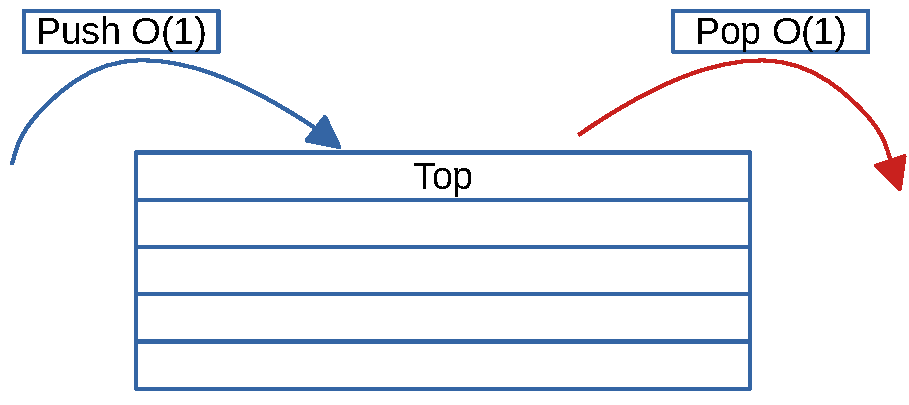
\includegraphics[scale=.6]{chapters/datastructures/images/stack_1.pdf}
		\caption[In a stack only the element at the top is modified.]{In a stack only the element at the top is modified.}
		\label{stack_1}
	\end{center}
\end{figure}

\begin{figure}[H]
\centering
\begin{tikzpicture}[draw, minimum width=1.5cm, minimum height=0.5cm, thick]
    \node[draw] (push) at (-1,2) {};
    \node[draw=none] at ($(push) + (0, 5mm)$) {Push $O(1)$};
    \node[draw] (pop) at (1,2) {};
    \node[draw=none] at ($(pop) + (0, 5mm)$) {Pop $O(1)$};
    
    \matrix (queue)[matrix of nodes, nodes={draw, nodes={draw}}, nodes in empty cells, row sep=-\pgflinewidth]
    {
       \\ \\ \\ \\
    };

    \draw[->, >=stealth] (0.25,1) -- (pop.south);
    \draw[->, >=stealth] (push.south) -- (-0.25,1);
\end{tikzpicture}
\caption[In a stack only the element at the top is modified.]{In a stack only the element at the top is modified.}
\label{stack_1}
\end{figure}

\subsection{Stack Implementation}
The following is the implementation in Python of a stack using the linked list.
\begin{lstlisting}[firstnumber=1, caption={Stack implementation.}]
class Element():
	...

class LinkedList():
	...
	
	def insert_first(self, new_element):
		new_element.next = self.head
		self.head = new_element
	
	def delete_first(self):
		if self.head:
			delete_element = self.head
			temp = deleted_element.next
			self.head = temp
			return deleted_element
		else:
			return None

class Stack():
	
	def __init__(self, top=None):
		self.ll = LinkedList(top)
		
	def push(self, new_element):
		self.ll.insert_first(new_element)
	
	def pop(self):
		self.ll.delete_first()
\end{lstlisting}

\section{Queue}
\label{queue}
A \textbf{queue} is abstract data type belonging to collections very similar to the stacks. For a queue the admitted operations are only on the oldest element, thus the first element to be added \cite{wikiqueue} (\href{https://en.wikipedia.org/wiki/Queue_(abstract_data_type)}{Queue, Wikipedia}). The allowed operations on a queue are:
\begin{itemize}
\item[•] \textbf{Enque}: adding an element at the bottom of the queue
\item[•] \textbf{Deque}: removing the element at the head of the queue
\item[•] \textbf{Pick}: observing the element at the head of the queue
\end{itemize}
For adding and removing operations the complexity remain constant. Queues are also called \textbf{First In, First Out} (\textbf{FIFO}). 

The most efficient way to implement a queue is using linked lists.

\begin{figure}[H]
	\begin{center}
		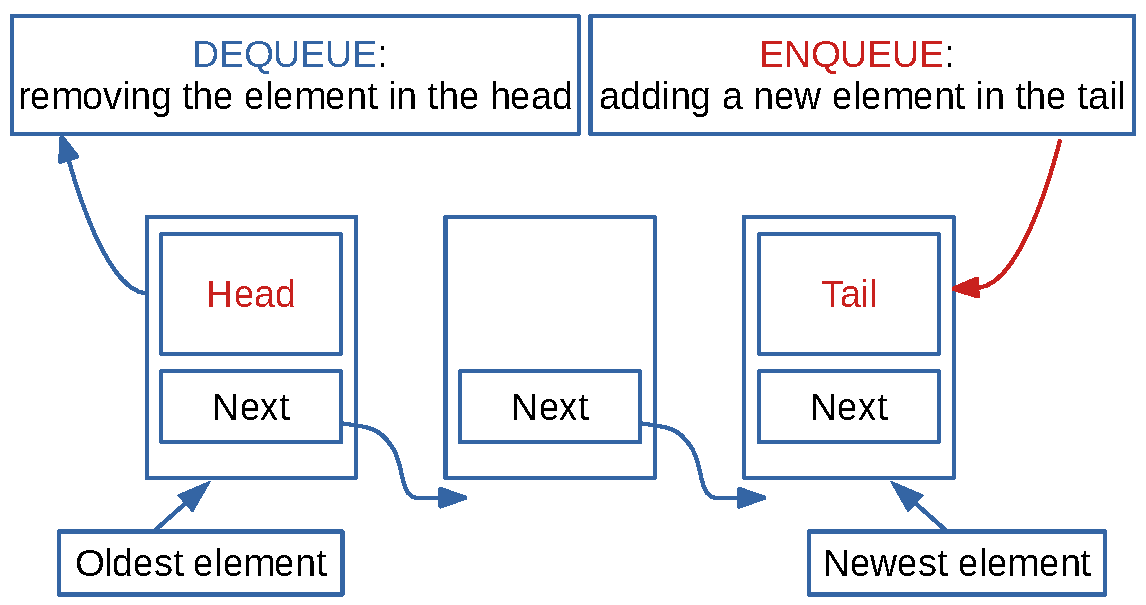
\includegraphics[scale=.6]{chapters/datastructures/images/queue_1.pdf}
		\caption[Allowed operations on queue elements.]{In a queue only the first element to be added can be removed or where a new element can be added.}
		\label{queue_1}
	\end{center}
\end{figure}

\begin{figure}[H]
\centering
\begin{tikzpicture}[draw, minimum width=1.5cm, minimum height=0.5cm, thick]  
    \node[draw] (enqueue) at (-1,2) {};
    \node[draw=none] at ($(enqueue) + (0, 5mm)$) {Enqueue $O(1)$};
    \node[draw] (dequeue) at (1,-2) {};
    \node[draw=none] at ($(dequeue) + (0, -5mm)$) {Dequeue $O(1)$};
    
    \matrix (queue)[matrix of nodes, nodes={draw, nodes={draw}}, nodes in empty cells, row sep=-\pgflinewidth]
    {
      Head \\ 
       \\ 
       \\ 
       Tail \\
    };

    \draw[->, >=stealth] (0.25,-1.05) -- (dequeue.north);
    \draw[->, >=stealth] (enqueue.south) -- (-0.25,1.05);
\end{tikzpicture}
\caption[Allowed operations on queue elements.]{In a queue only the first element to be added can be removed or where a new element can be added.}
\label{queue_1}
\end{figure}

A generalization of queues and linked lists are \textbf{deques}, in which is possible to perform deque and enque operations on both the \textbf{head} and \textbf{tail}.

\begin{figure}[H]
	\begin{center}
		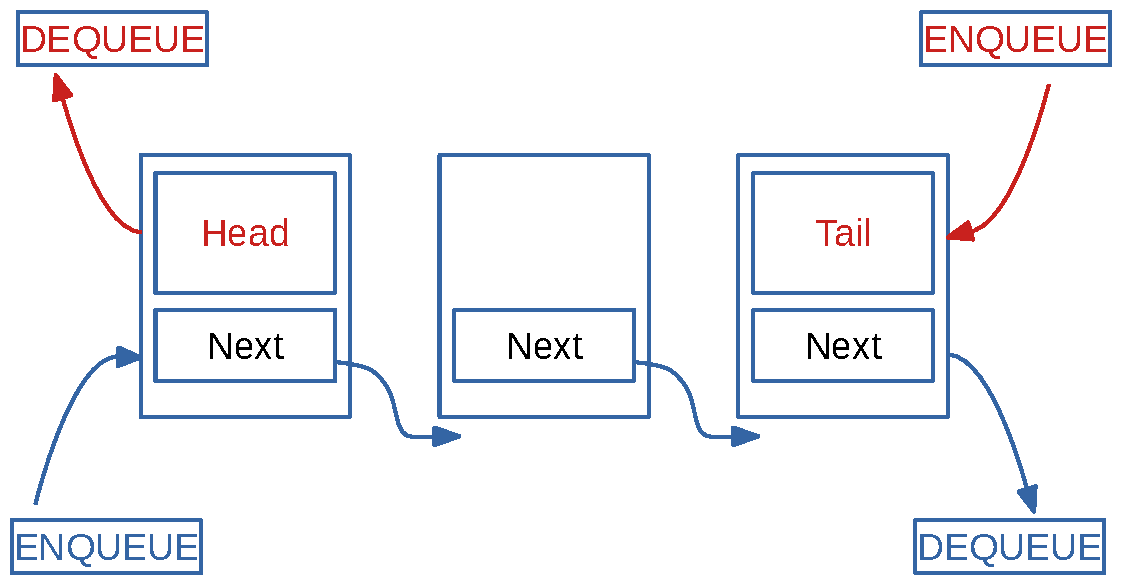
\includegraphics[scale=.6]{chapters/datastructures/images/queue_2.pdf}
		\caption[In a deque the operations can be done on both head and tail.]{In a deque the operations can be done on both head and tail.}
		\label{queue_2}
	\end{center}
\end{figure}

\begin{figure}[H]
\centering
\begin{tikzpicture}[draw, minimum width=1.5cm, minimum height=0.5cm, thick]  
    \node[draw] (enqueue) at (-1.5,2) {};
    \node[draw=none] at ($(enqueue) + (0, 5mm)$) {Enqueue $O(1)$};
    \node[draw] (dequeue1) at (1.5,2) {};
    \node[draw=none] at ($(dequeue1) + (0, 5mm)$) {Dequeue $O(1)$};
    
    \node[draw] (dequeue) at (1.5,-2) {};
    \node[draw=none] at ($(dequeue) + (0, -5mm)$) {Dequeue $O(1)$};
    \node[draw] (enqueue1) at (-1.5,-2) {};
    \node[draw=none] at ($(enqueue1) + (0, -5mm)$) {Enqueue $O(1)$};
    
    \matrix (queue)[matrix of nodes, nodes={draw, nodes={draw}}, nodes in empty cells, row sep=-\pgflinewidth]
    {
      Head \\ 
       \\ 
       \\ 
       Tail \\
    };

    \draw[->, >=stealth] (0.25,-1.052) -- (dequeue.north);
    \draw[->, >=stealth] (enqueue.south) -- (-0.25,1.05);
    
    \draw[->, >=stealth] (enqueue1.north) -- (-0.25,-1.05);
    \draw[->, >=stealth] (0.25,1.05) -- (dequeue1.south);
\end{tikzpicture}
\caption[In a deque the operations can be done on both head and tail.]{In a deque the operations can be done on both head and tail.}
\label{queue_2}
\end{figure}

Another modification of queue are \textbf{priority queue}, in which each element has a priority (a numeric value that indicates its importance). When an element of the queue is removed (deque), the element to be removed is the one which has the highest priority. In case two or more elements have the same priority the oldest element is removed.

\begin{figure}[H]
	\begin{center}
		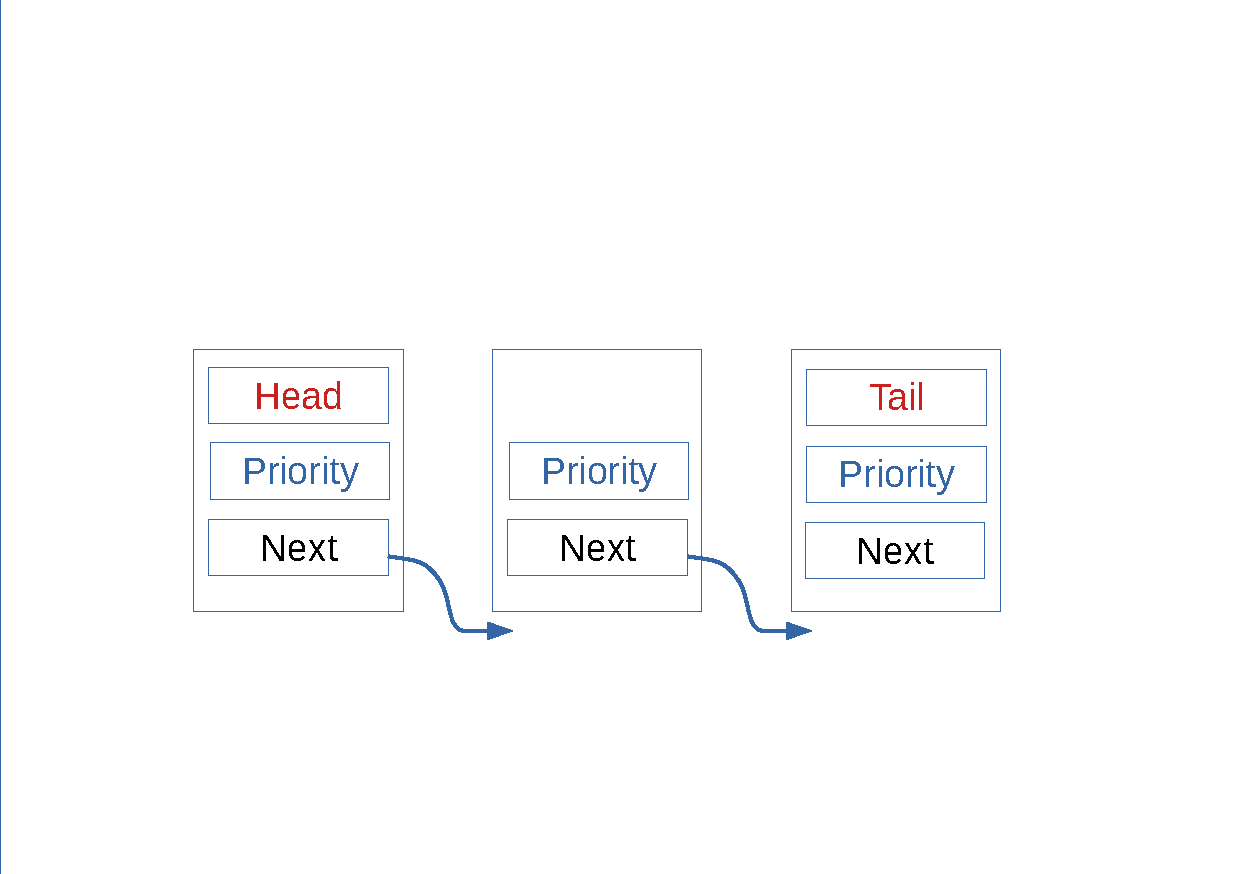
\includegraphics[scale=.6]{chapters/datastructures/images/queue_3.pdf}
		\caption[A priority queue.]{A priority queue.}
		\label{queue_3}
	\end{center}
\end{figure}

\begin{figure}[H]
\centering
\begin{tikzpicture}[draw, minimum width=2.7cm, minimum height=0.5cm, thick]  

    \matrix (queue)[matrix of nodes, nodes={draw, nodes={draw}}, nodes in empty cells, row sep=-\pgflinewidth]
    {
      Head, Priority \\ 
       \\
       \\
       \\
      Tail, Priority \\
    };

\end{tikzpicture}
\caption[A priority queue.]{A priority queue.}
\label{queue_3}
\end{figure}

\subsection{Queue Implementation}
The following is the implementation of a queue using the list of Python.
\begin{lstlisting}[firstnumber=1, caption={Queue implementation.}]
class Queue():
	def __init__(self, head=None):
		self.storage = [head]
	
	def enqueue(self, new_element):
		self.storage.append(new_element)
	
	def peek(self):
		return self.storage[0]
	
	def dequeue(self):
		return self.storage.pop(0)
\end{lstlisting}

\section{Set}
A \textbf{set} is an abstract data type in which the unique values are stored without a particular order \cite{wikiset} (\href{https://en.wikipedia.org/wiki/Set_(abstract_data_type)}{Set, Wikipedia}).

\section{Map}
A \textbf{map}, \textbf{associative array}, \textbf{symbol table}, or \textbf{dictionary} is an abstract data type composed of a collection of (key, value) pairs \cite{wikihashmap} (\href{https://en.wikipedia.org/wiki/Associative_array}{Hash Map, Wikipedia}). The group of the key is a set, in which each element has a unique value. Map is a very useful data type, used in a lot of situations. 

\begin{figure}[H]
	\begin{center}
		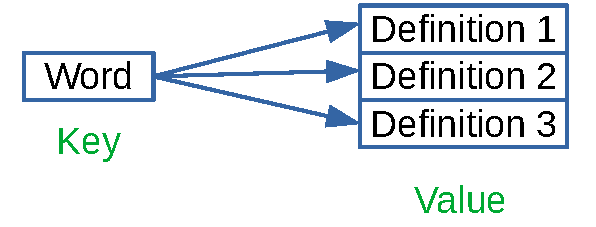
\includegraphics[scale=.6]{chapters/datastructures/images/map_1.pdf}
		\caption[An example of a map.]{An example of a map.}
		\label{map_1}
	\end{center}
\end{figure}

\begin{figure}[H]
\centering
\begin{tikzpicture}[draw, minimum width=2.4cm, minimum height=0.5cm, thick]  

    \matrix [matrix of nodes, nodes={draw, nodes={draw}}, nodes in empty cells, row sep=-\pgflinewidth] (queue)
    {
      Definition $1$ \\ 
      Definition $2$ \\
      Definition $3$ \\
    };
    
    \node[rectangle, draw, minimum width=1cm, minimum height=0.5cm] (word) at ($(queue) + (-3.6,0)$) {Word};
    
    \node[draw=none] (key) at ($(word) + (0,-8mm)$) {\textcolor{ForestGreen}{Key}};
    \node[draw=none] (key) at ($(queue) + (0,-14mm)$) {\textcolor{ForestGreen}{Value}};
    
    \draw[->, >=stealth] (word.east) -- (queue-1-1.west);
    \draw[->, >=stealth] (word.east) -- (queue-2-1.west);
	\draw[->, >=stealth] (word.east) -- (queue-3-1.west);    
    
\end{tikzpicture}
\caption[An example of a map.]{An example of a map.}
\label{map_1}
\end{figure}

\section{Hash Table}
A \textbf{hash table} or \textbf{hash map} is a data structure that implements the map abstract data type \cite{wikihashtable} (\href{https://en.wikipedia.org/wiki/Hash_table}{Hash Table, Wikipedia}). Hash table uses the \textbf{hash function} for working \cite{wikihashfunction} (\href{https://en.wikipedia.org/wiki/Hash_function}{Hash Function, Wikipedia}). Using the hash function is called hashing.

\subsection{Hashing}
Hashing is an operation that allows to transform the value of a variable to another one which is much easier to find within a collection. If we want to find a value inside a collection (list, stack, queue, etc) the time requested for the search is linear with the size of the collection. In fact we have to check all the elements until the searched one is found (in case of stack and queue this is not true is only the last or the first element respectively is checked). For solving this problem and thus to find an element in a constant time hash function are used. 

Let us consider the follow example, where we have an array in which we would like to store big random numbers. A simple way for hashing these numbers is to consider only the last numbers (56 and 17) and divide them for a fixed number. The reminder of the division is used as the new index of the array associated to the number (Figure ).

What happen when the hash function transforms two different number in the same? In this case we have a \textbf{collision}. In case of a collision there are several strategies for solving this issue: one way could be to change the the hash function, another one could be to use an array for storing different values associated to the same key (\textbf{bucket}). For the last occurrence the worst case complexity for a search is \(O(n)\) (Figure \ref{map_2}).

\begin{figure}[H]
	\begin{center}
		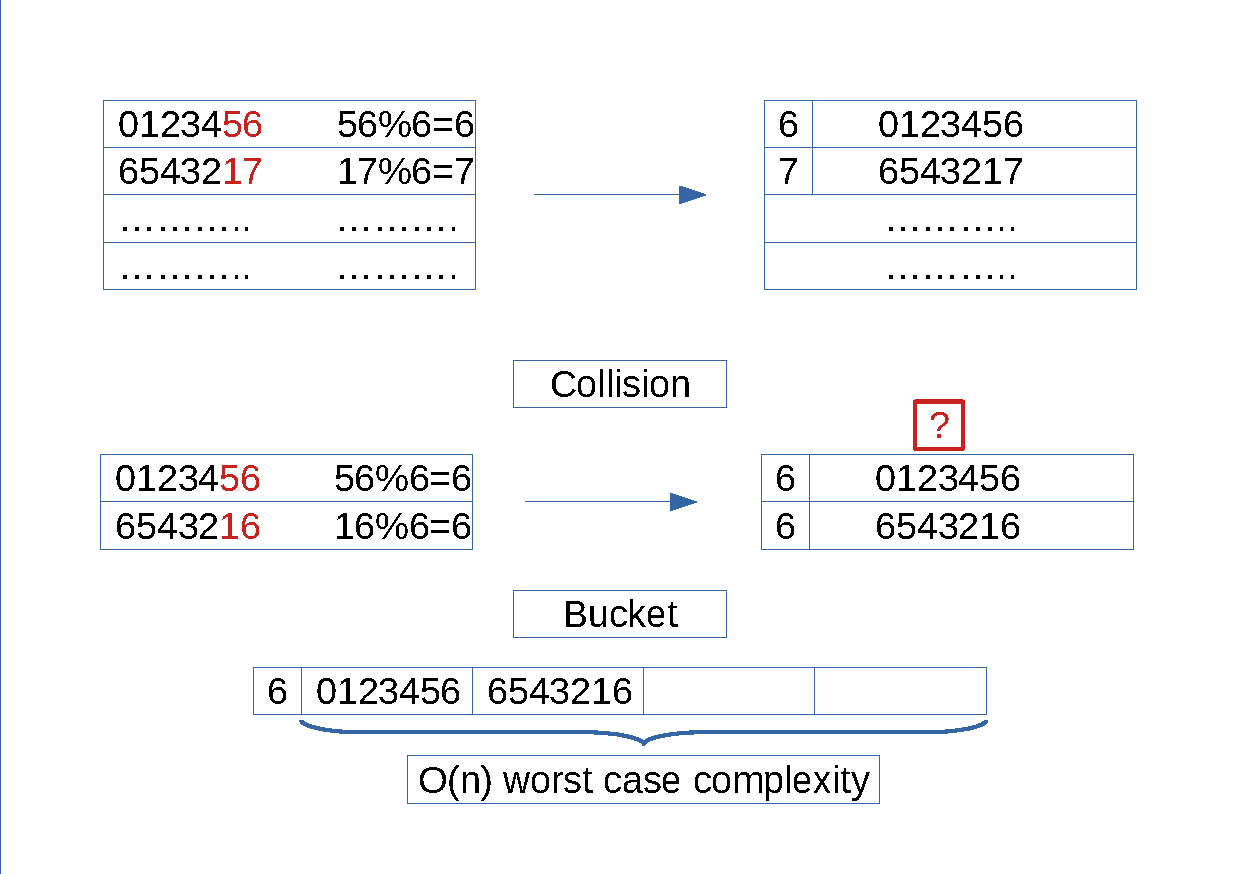
\includegraphics[scale=.6]{chapters/datastructures/images/map_2.pdf}
		\caption[An example of collision and a possible way to solve this issue by using the bucket method.]{An example of collision and a possible way to solve this issue by using the bucket method.}
		\label{map_2}
	\end{center}
\end{figure}

\begin{figure}[H]
\centering
\begin{tikzpicture}[draw, minimum width=4.2cm, minimum height=0.5cm, thick, align=center]  

    \matrix [matrix of nodes, nodes={draw, nodes={draw}}, nodes in empty cells, row sep=-\pgflinewidth] (tab1)
    {
      $01234\textcolor{BrickRed}{56} \qquad 56\%6=6$ \\ 
      $65432\textcolor{BrickRed}{17} \qquad 17\%6=7$ \\
      ... \qquad ... \\
      ... \qquad ... \\
    };
    
    \matrix [matrix of nodes, nodes={draw, nodes={draw}}, nodes in empty cells, row sep=-\pgflinewidth, minimum width=3cm, minimum height=0.5cm] (tab2) at ($(tab1) + (7.6,0)$)
    {
      $6 -> 0123456$ \\ 
      $7 -> 6543217$ \\
      ... \qquad ... \\
      ... \qquad ... \\
    };
    
    \draw[->, >=stealth] (tab1) -- (tab2);
    
    
    \draw (3.6,-2) node[draw=none, rectangle, align=left] (collision) {Collision};
    
    \matrix [matrix of nodes, nodes={draw, nodes={draw}}, nodes in empty cells, row sep=-\pgflinewidth] (tab3) at ($(tab1) + (0,-3)$)
    {
      $01234\textcolor{BrickRed}{56} \qquad 56\%6=6$ \\ 
      $65432\textcolor{BrickRed}{16} \qquad 16\%6=6$ \\
    };
    
    \matrix [matrix of nodes, nodes={draw, nodes={draw}}, nodes in empty cells, row sep=-\pgflinewidth, minimum width=3cm, minimum height=0.5cm] (tab4) at ($(tab3) + (7.6,0)$)
    {
      $6 -> 0123456$ \\ 
      $6 -> 6543216$\\
    };
    \draw ($(tab4.north) + (0,2mm)$) node[draw, rectangle, align=left, BrickRed, minimum width=0.5cm, minimum height=0.5cm] {?};
    
    \draw[->, >=stealth] (tab3) -- (tab4);
    
    \draw (3.6,-4) node[draw=none, rectangle, align=left] {Bucket};
        
    \matrix [matrix of math nodes, nodes={draw, nodes={draw}, anchor=center}, nodes in empty cells, row sep=-\pgflinewidth, minimum width=0.5cm, minimum height=0.6cm, column sep=-\pgflinewidth] (tab5) at ($(tab3) + (3.6,-1.6)$)
    {
      $6$ & $0123456$ & $6543216$ & ... & $n$ \\
    };
    \draw ($(tab5) + (0,-7mm)$) node[draw=none, rectangle, align=left]  {$O(n)$ worst case complexity};

\end{tikzpicture}
\caption[An example of collision and a possible way to solve this issue by using the bucket method.]{An example of collision and a possible way to solve this issue by using the bucket method.}
\label{map_2}
\end{figure}

It does not exist a perfect hash function and a trade off must always be reached. A way to analyse a hash function is by using the \textbf{load factor} defined as follow: \(Load \ Factor = \# \ of \ entries / \ \# \ of \ buckets\). For example, if we want to save 10 values using 1000 buckets the Load Factor is equal to 0.01, and most of the buckets is empty. In this case is convenient to change the hash function by using less buckets. More the Load Factor is closed to 0 more the hash table will be empty (\textbf{sparse}), and more the Load Factor is closed to 1 more the has table will be full and efficient. In case the Load Factor is bigger than 1 there is the certainty there will happen some collisions.
Another example: let us consider a hash function that divide the numbers by 100. If we consider 100 values all multiple of 5, the Load Factor will be: \(Load \ Factor = \# \ of \ entries / \ \# \ of \ buckets = 100/100 = 1\). But this way is very slow and a different configuration should be used to make this more efficient. For example if we use more bucket, for example 107, we still avoid collisions and we do not have the hash map too much sparse.

\section{String Keys}
Let us consider a hash function that associates a word to a numerical value. For example we can use the ASCII character encoding of the first two letters of the string as numerical value. Thus, in case of \textit{UDACIY} we have \textit{U}=85 and \textit{D}=68. For hash function we can use the following: \(S\left[0\right] * 31^{(n-1)} + S\left[1\right] * 31^{(n-2)} + \ldots + S\left[n-1\right]\), where \(n\) is the length of the string. In this way for the word in the previous example, in which only the first two letters are encoded in a numerical value for simplicity, we have \(85*31^{1} + 68 = 2703\).

This hash function works very well because it assures a very low probability of collision. \(31\) is a number empirically obtained by several researches and showed good results in hashing strings.

\subsection{String Keys Implementation}
The following is the implementation of the string key map in Python.

The hash function of this implementation is: \(Hash \ Function = (ASCII[0]*100) + ASCII[1]\). In this code \textit{ord()} and \textit{char()} functions are used. \textit{ord()} takes a char as an argument and return the respective ASCII code (\(ord('U')=85\)), and \textit{char()} takes a numeric value as ASCII code and return the respective char (\(char(85)='U'\)).
\begin{lstlisting}[firstnumber=1, caption={String key implementation.}]
class HashTable():
	def __init__(self):
		self.table = [None]*10000
	
	def store(self, string):
		hv = self.calculate_hash_value(string)
		if hv != -1:
			if self.table[hv] != None:
				self.table[hv].append(string)
			else:
				self.table[hv] = [string]
	
	def lookup(self, string):
		hv = self.calculate_hash_value(string)
		if hv != -1:
			if self.table[hv] != None:
				if string in self.table[hv]:
					return hv
		return -1
	
	def calculate_hash_value(self, string):
		value = ord(string[0]*100) + ord(string[1])
		return value
\end{lstlisting}